\chapter*{Hong Kong\markboth{Hong Kong}{}}
\section*{30 octobre 2015}
Je tente de passer la frontière entre la Chine et HK en vélo mais c'est impossible, obligé de mettre le vélo dans un bus. 

 Belles pistes cyclables sur quelques dizaines de km ensuite.
\begin{center} 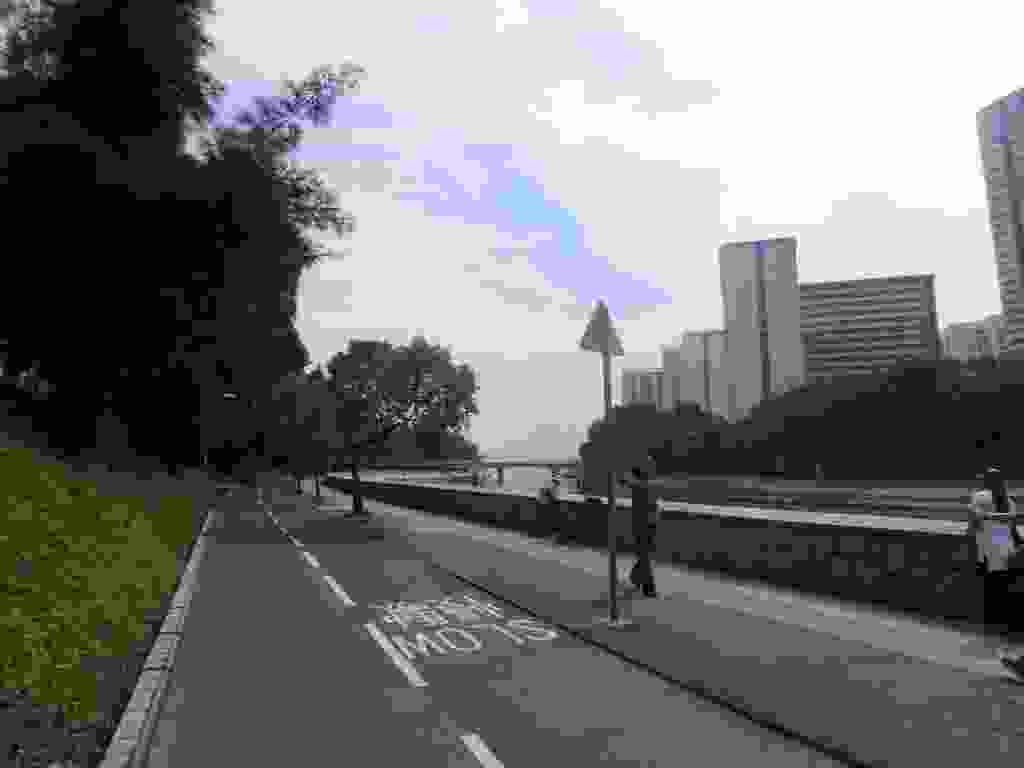
\includegraphics[width=\mywidth]{../wp-content/uploads/2015/10/wpid-oi000043-1024x768.jpg} \end{center}
\vspace{-\topsep}
\pagebreak

~\\~\\
\vspace{2mm}
\vfill
\begin{center} 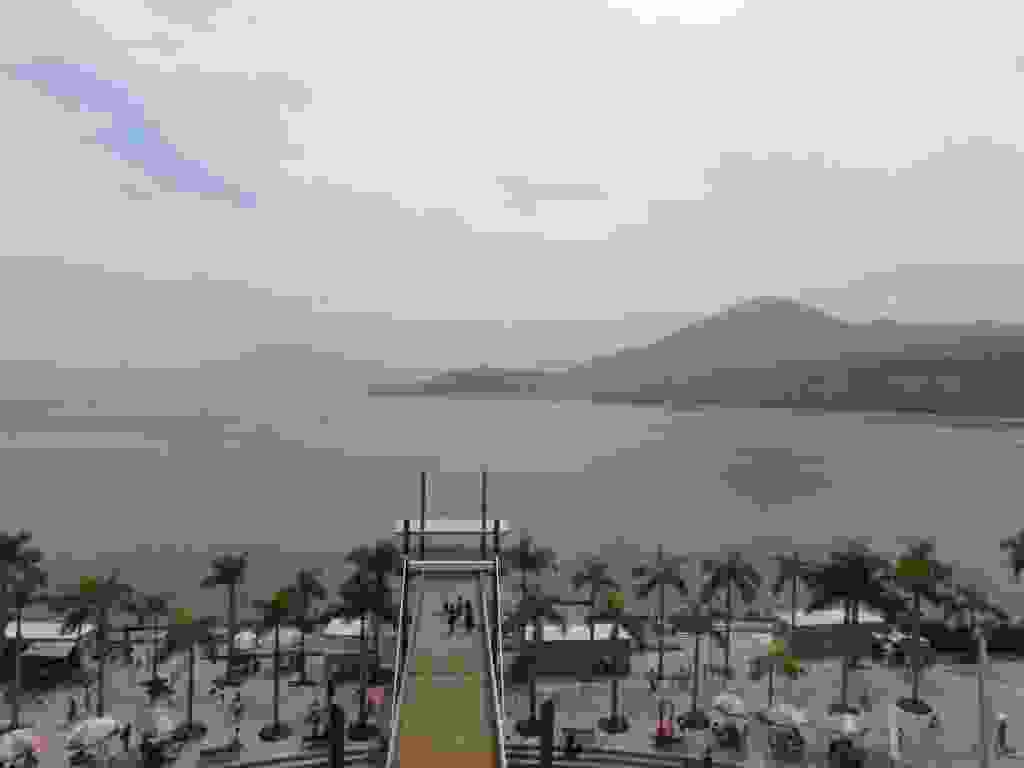
\includegraphics[width=\mywidth]{../wp-content/uploads/2015/10/wpid-oi000045-1024x768.jpg} \end{center}
\vfill
\begin{center} 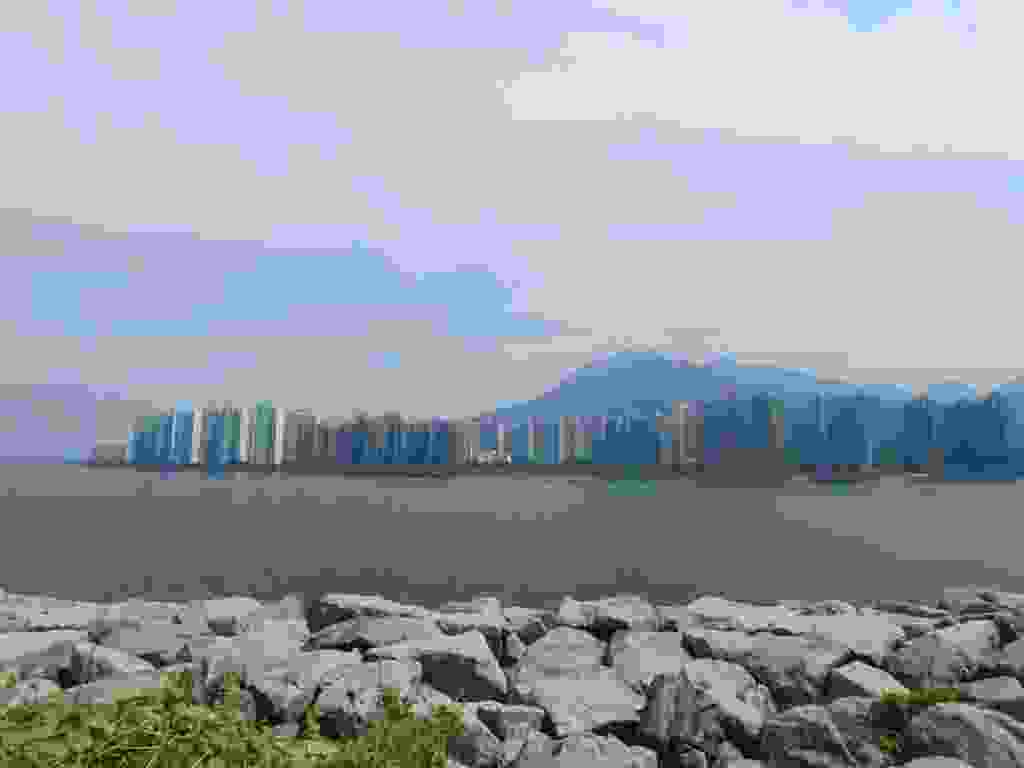
\includegraphics[width=\mywidth]{../wp-content/uploads/2015/10/wpid-oi000048-1024x768.jpg} \end{center}
\vspace{-\topsep}
\vspace{-0.75mm}
\pagebreak

  Premier jour dans le parc de Sai Kung à l'est des Nouveaux Territoires, partie de HK sur le continent. Forêts, petites plages et emplacements de camping gratuits, avec un climat parfait à cette saison. 
\begin{center} 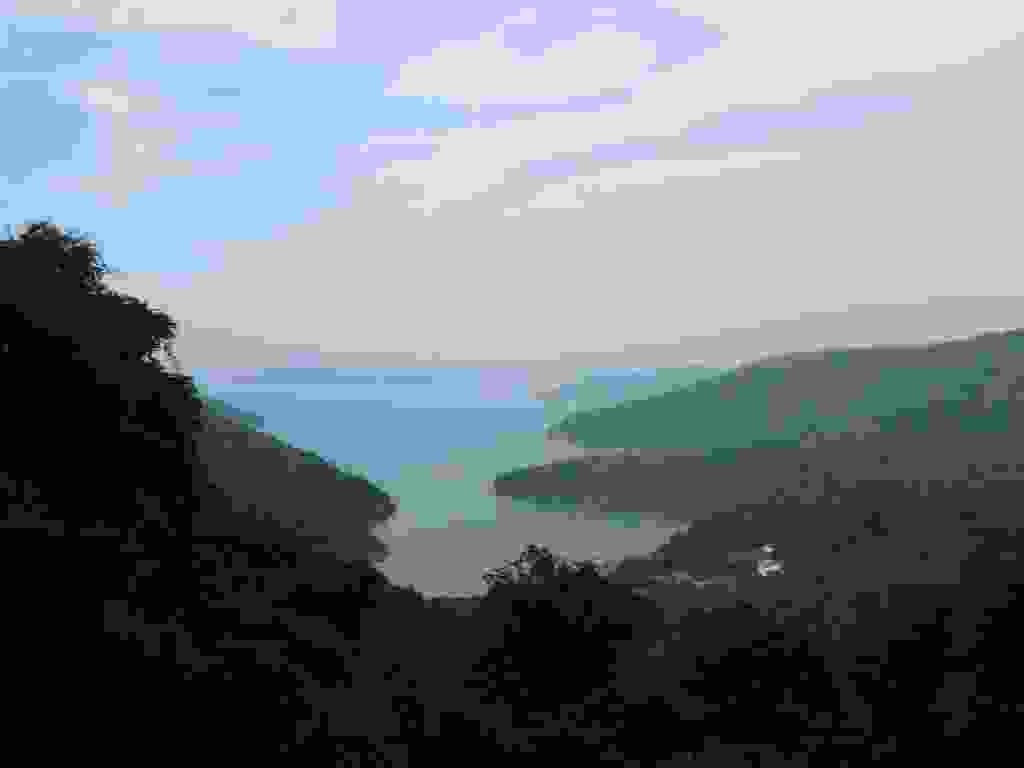
\includegraphics[width=\mywidth]{../wp-content/uploads/2015/10/wpid-oi000053-1024x768.jpg} \end{center}
\begin{center} 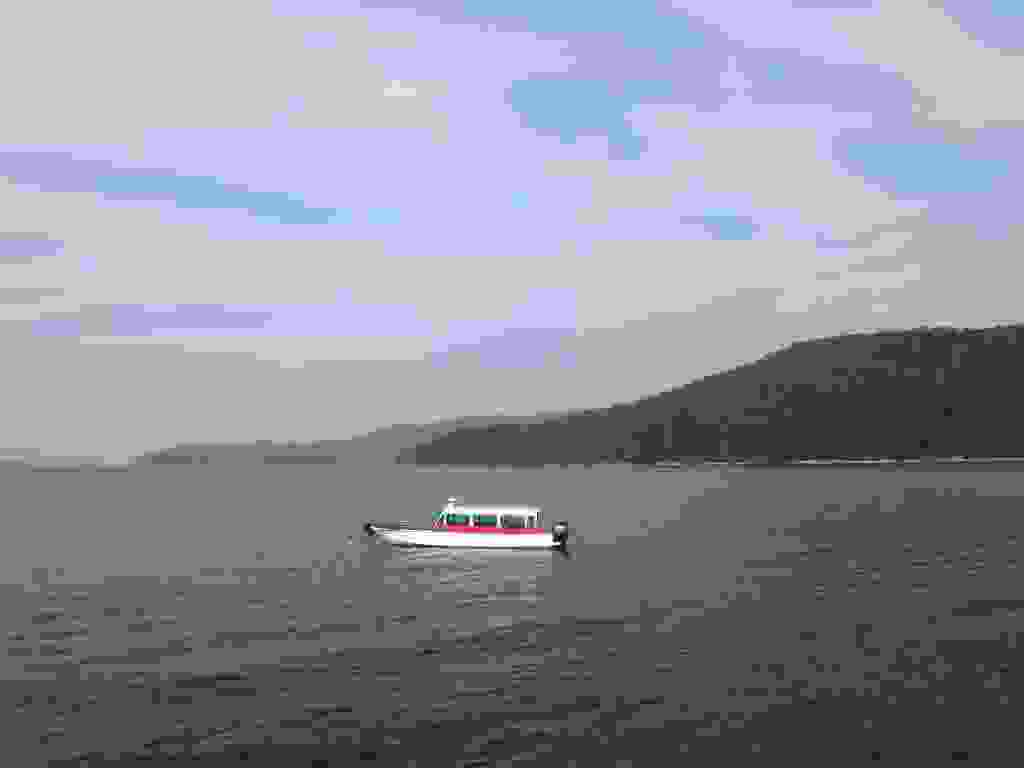
\includegraphics[width=\mywidth]{../wp-content/uploads/2015/10/wpid-oi000054-1024x768.jpg} \end{center}
\vspace{-\topsep}
\vspace{-2.25mm}
\pagebreak

~
\vspace{0.75mm}
\begin{center} 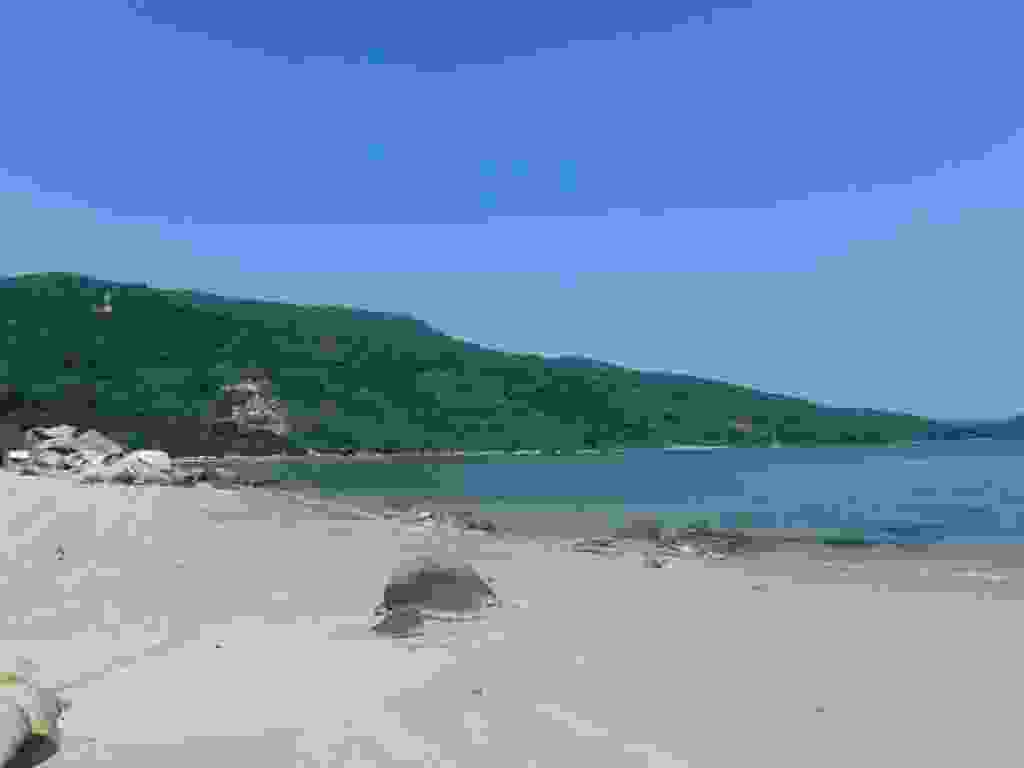
\includegraphics[width=\mywidth]{../wp-content/uploads/2015/10/wpid-oi000058-1024x768.jpg} \end{center}
\begin{center} 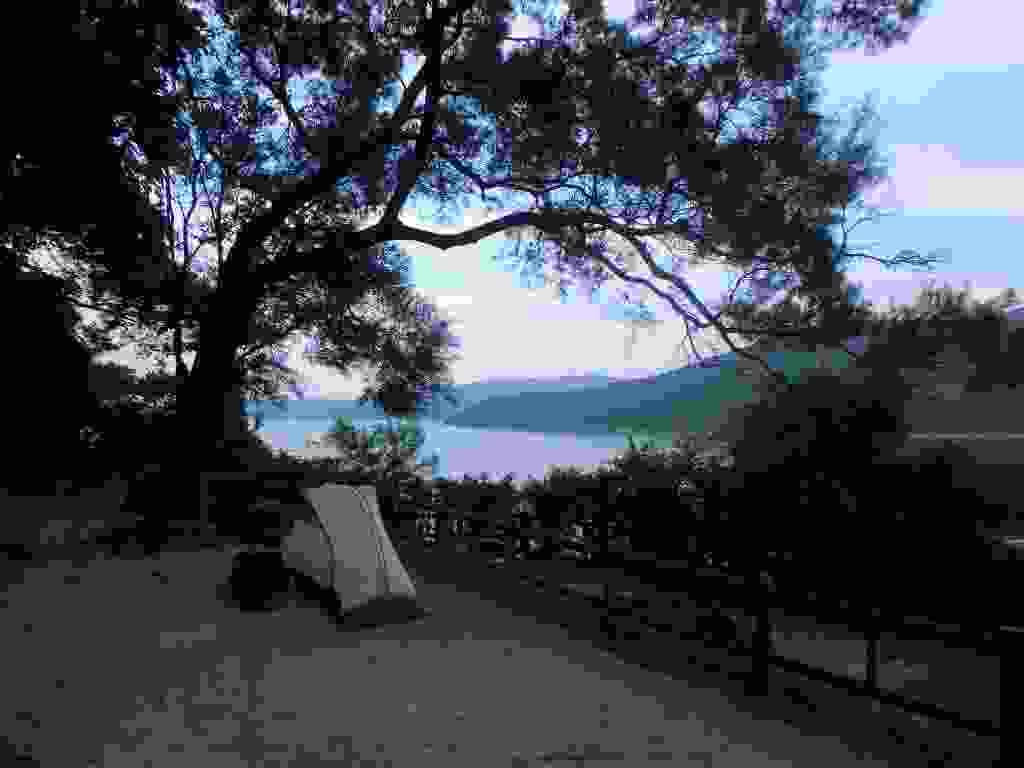
\includegraphics[width=\mywidth]{../wp-content/uploads/2015/10/wpid-oi000057-1024x768.jpg} \end{center}

~\\

\pagebreak
 
 Port de Sai Kung. 
\begin{center} 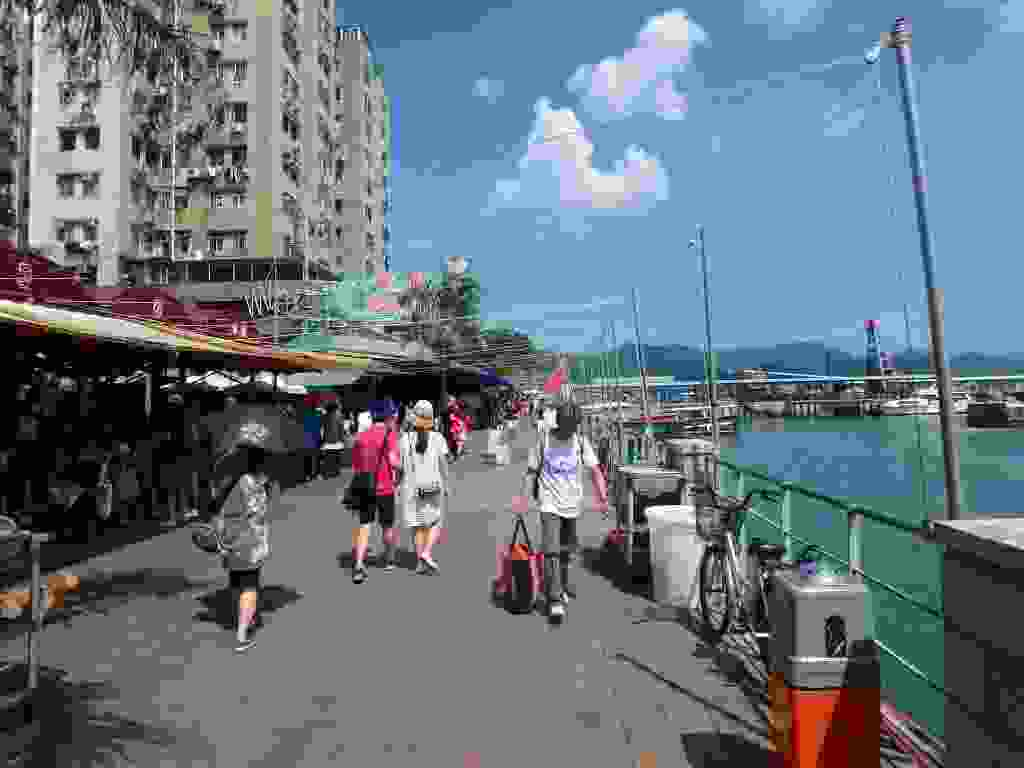
\includegraphics[width=\mywidth]{../wp-content/uploads/2015/10/wpid-oi000063-1024x768.jpg} \end{center}
\begin{center} 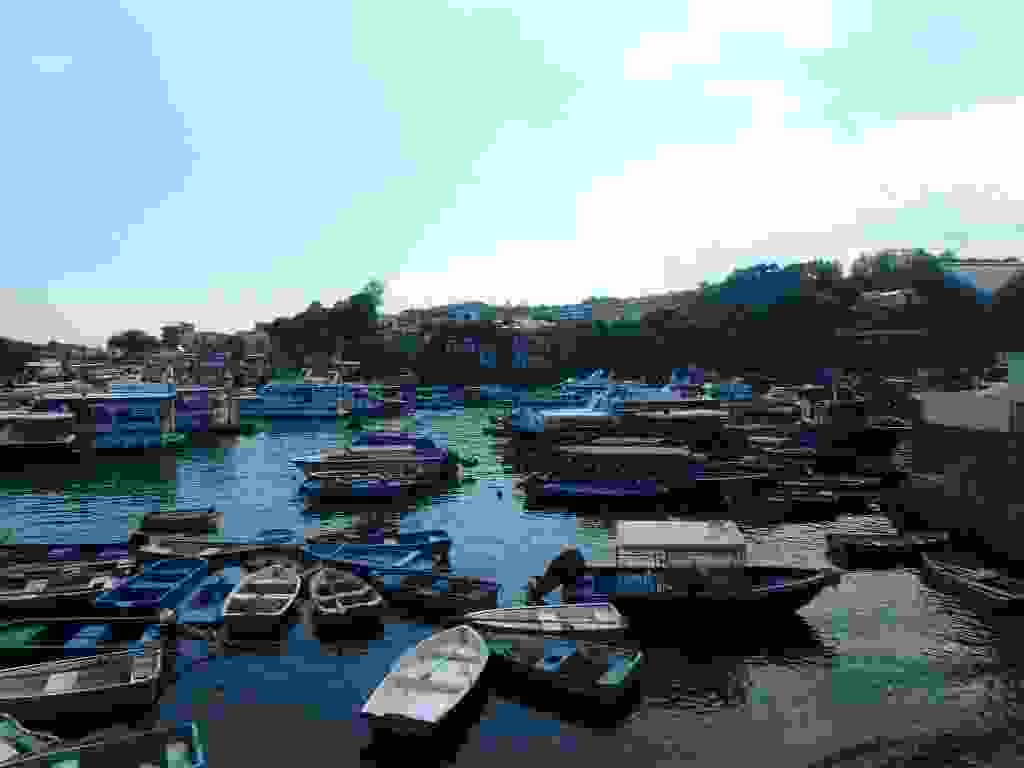
\includegraphics[width=\mywidth]{../wp-content/uploads/2015/10/wpid-oi000065-1024x768.jpg} \end{center}

 Je rejoins le centre, échangeurs énormes, routes surélevées dans tous les sens, certaines interdites aux vélos, le GPS est bien utile.
\pagebreak
 
 2 jours à l'hôtel dans le quartier de Kowloon, au 11\ieme\ étage d'un immeuble. Tellement exigu que le vélo doit rester dehors. 
\begin{center} 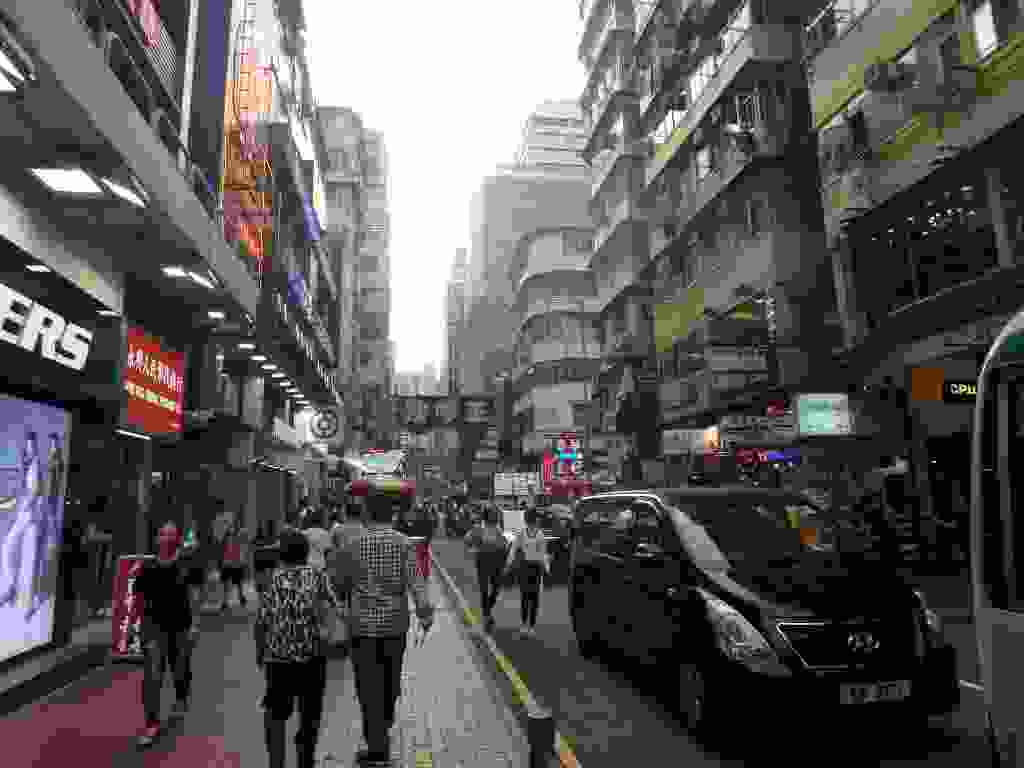
\includegraphics[width=\mywidth]{../wp-content/uploads/2015/10/wpid-oi000069-1024x768.jpg} \end{center}
~\\~\\
\begin{center} 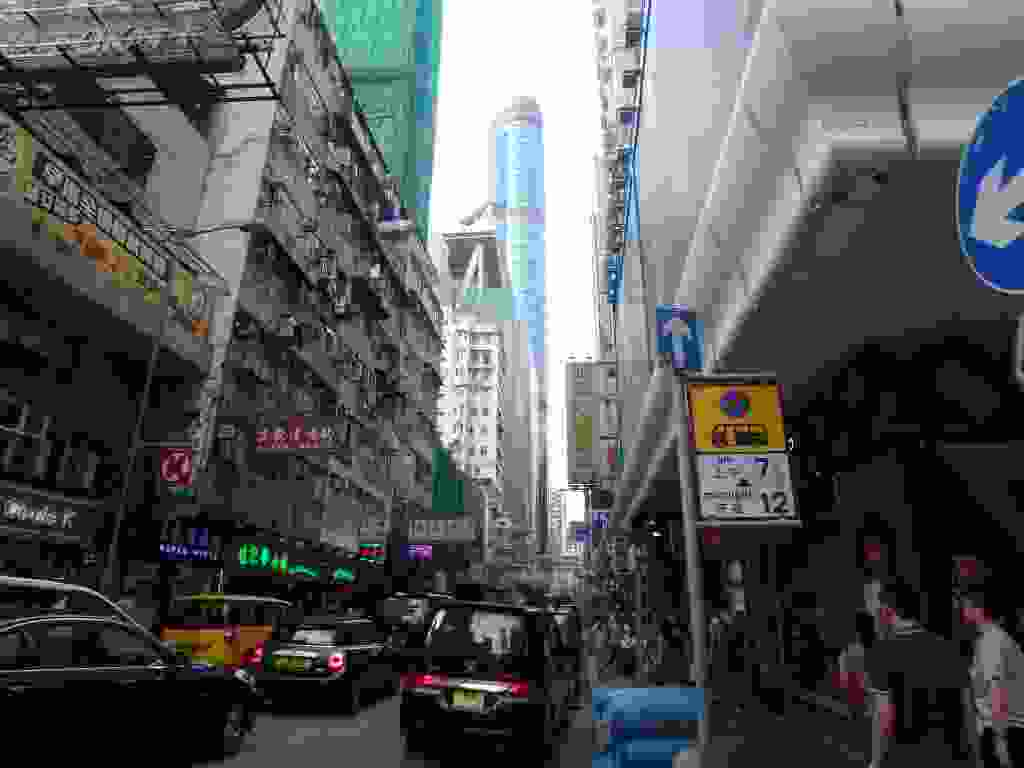
\includegraphics[width=\mywidth]{../wp-content/uploads/2015/10/wpid-oi0001201-1024x768.jpg} \end{center}
\vspace{-\topsep}
\pagebreak

~\\
\vspace{0.75mm}
\begin{center} 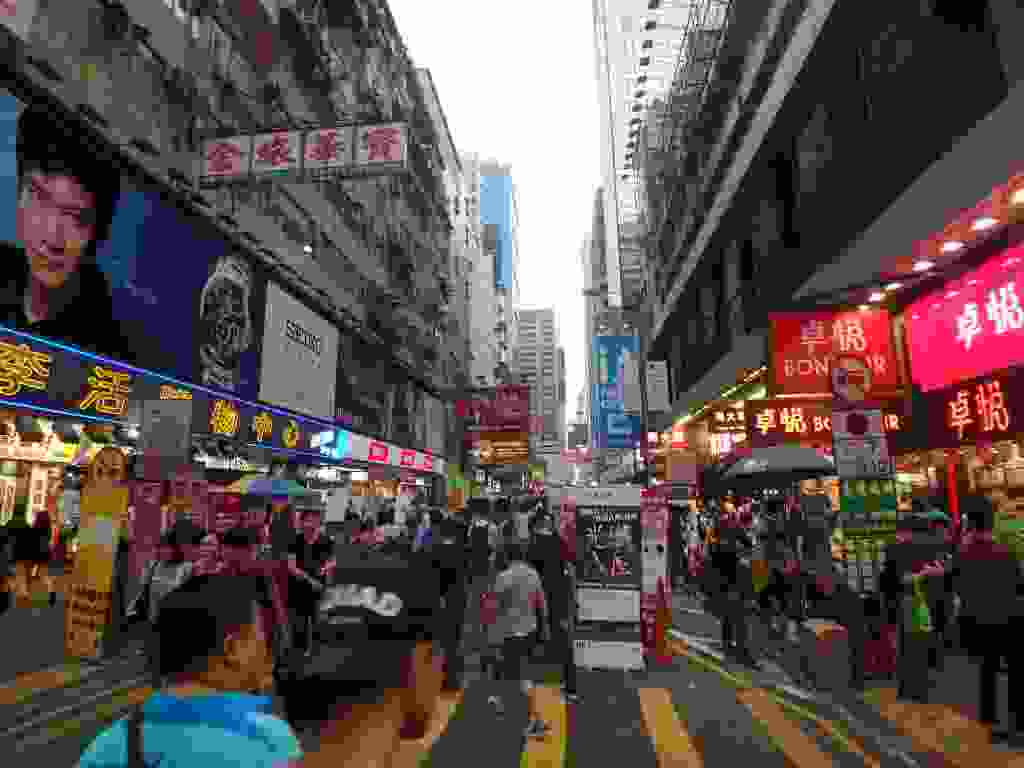
\includegraphics[width=\mywidth]{../wp-content/uploads/2015/10/wpid-oi0001221-1024x768.jpg} \end{center}

 Ensuite, Kévin m'héberge en couchsurfing dans l'appartement où il vit avec sa mère et son frère, superbe accueil avec un bon repas de spécialités locales. 
\begin{center} 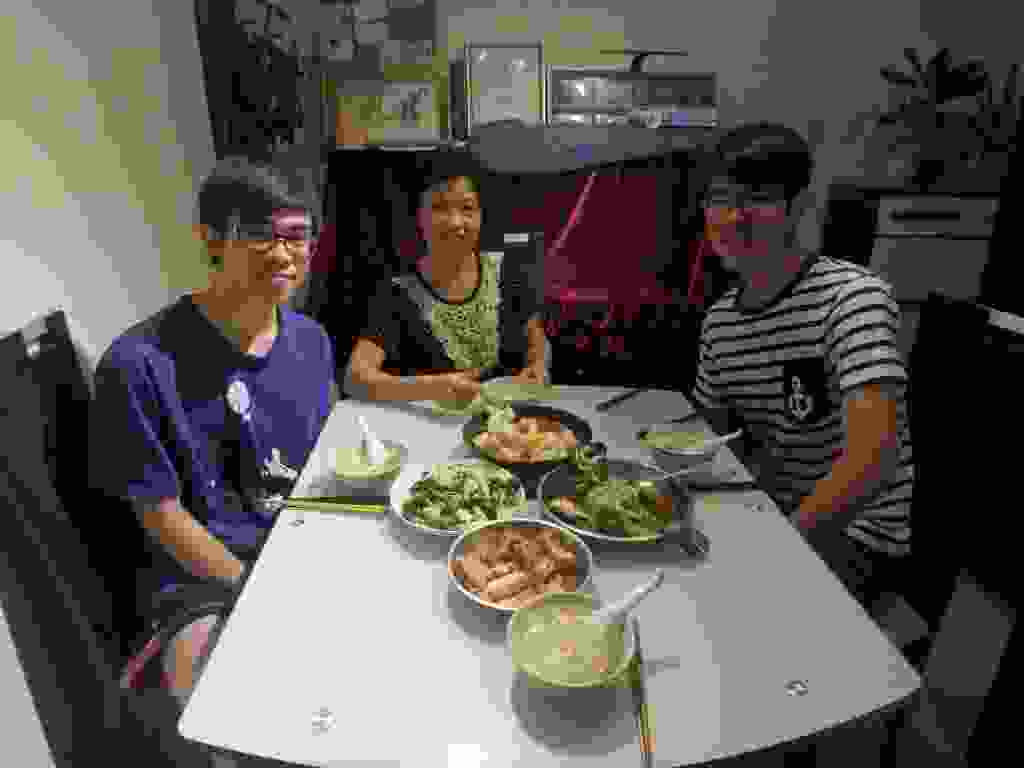
\includegraphics[width=\mywidth]{../wp-content/uploads/2015/10/wpid-oi000082-1024x768.jpg} \end{center}
\vspace{-\topsep}
\pagebreak
 
 On va sur l'île de Hong Kong, montée à Victoria Peak. 
\begin{center} 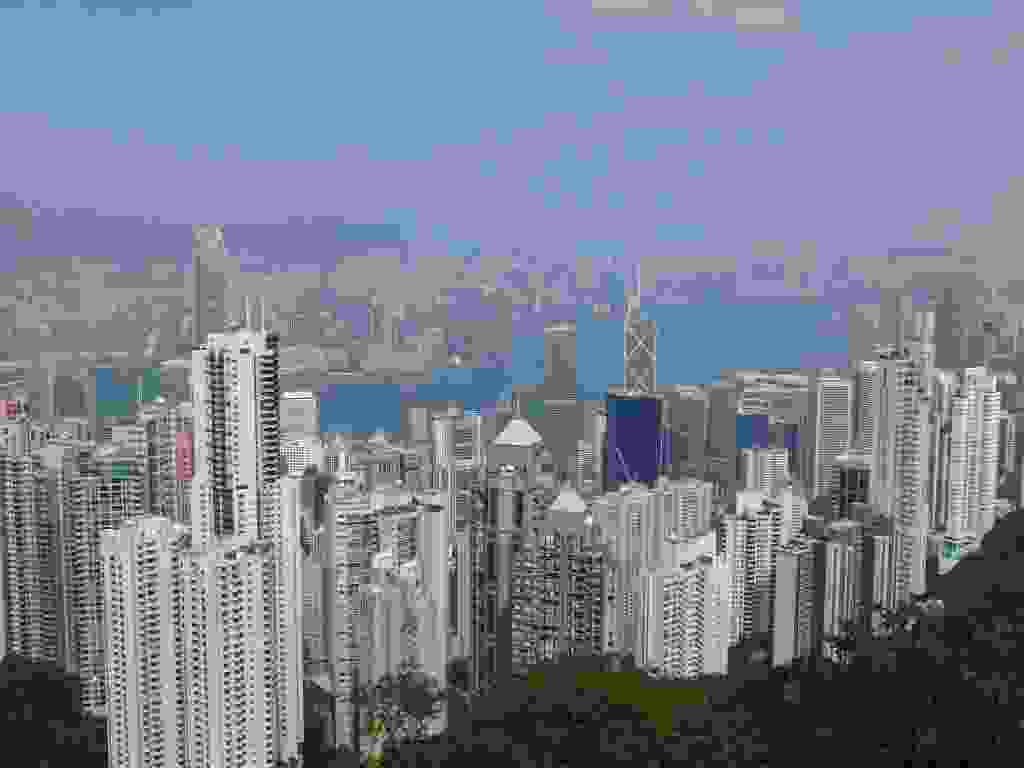
\includegraphics[width=\mywidth]{../wp-content/uploads/2015/10/wpid-oi000090-1024x768.jpg} \end{center}

 Balade pour voir le port d'Aberdeen au sud. 
\begin{center} 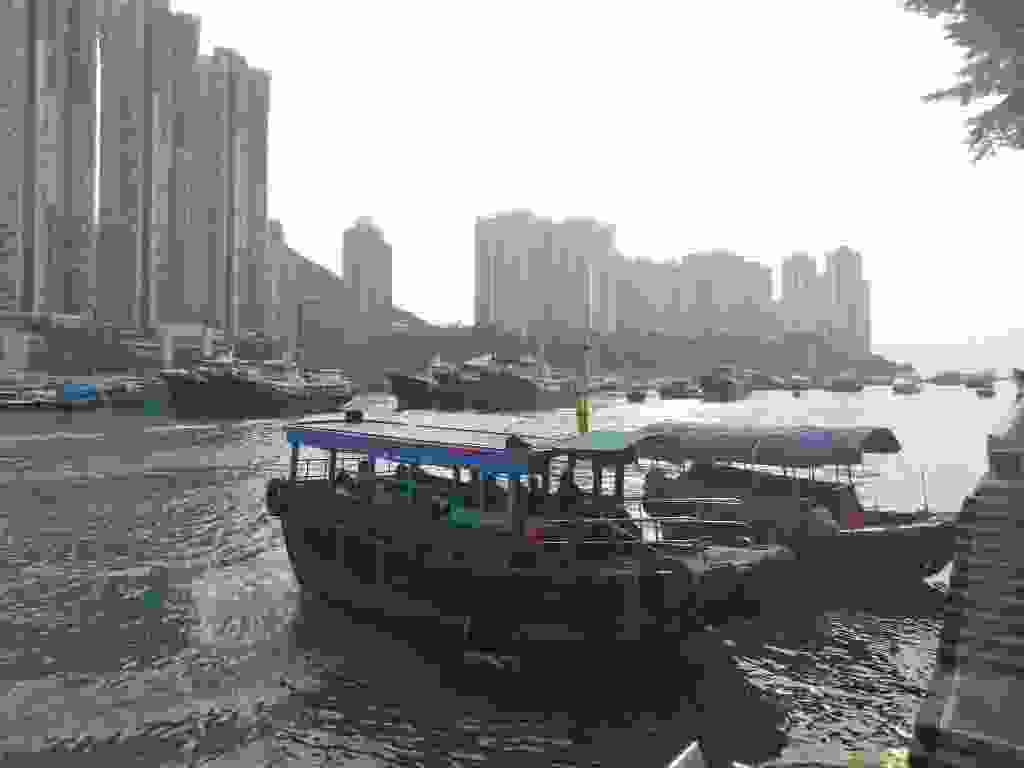
\includegraphics[width=\mywidth]{../wp-content/uploads/2015/10/wpid-oi000098-1024x768.jpg} \end{center}
\vspace{-\topsep}
\pagebreak
~
\vspace{0.25mm}
\begin{center} 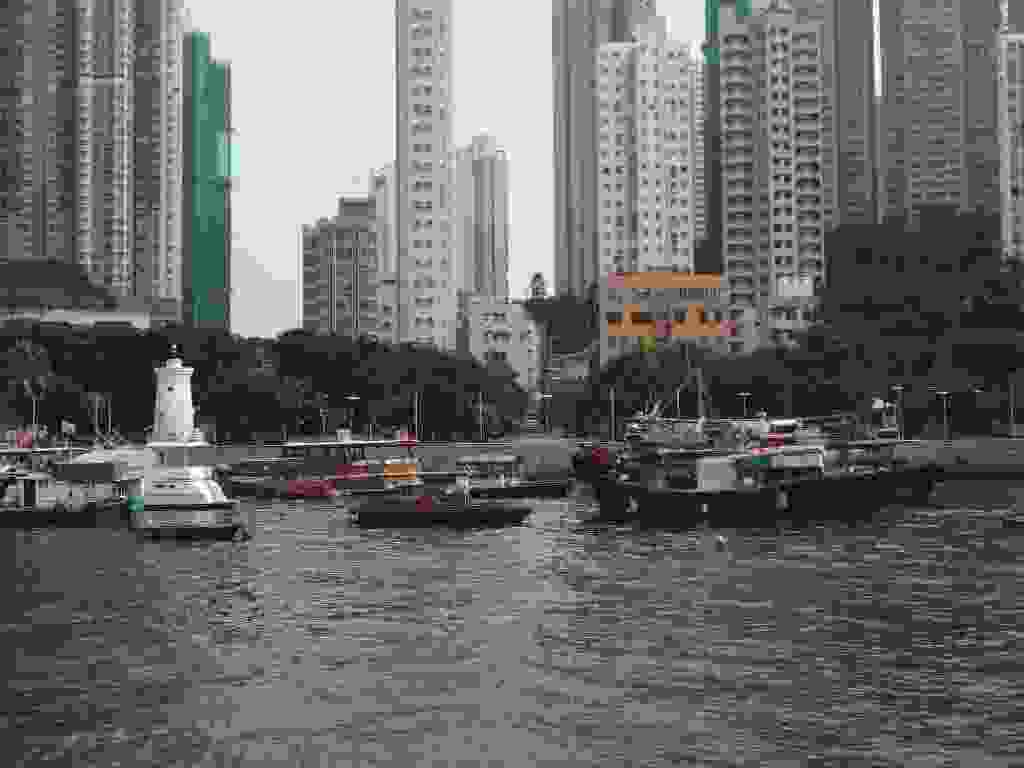
\includegraphics[width=\mywidth]{../wp-content/uploads/2015/10/wpid-oi000096-1024x768.jpg} \end{center}
~
\begin{center} 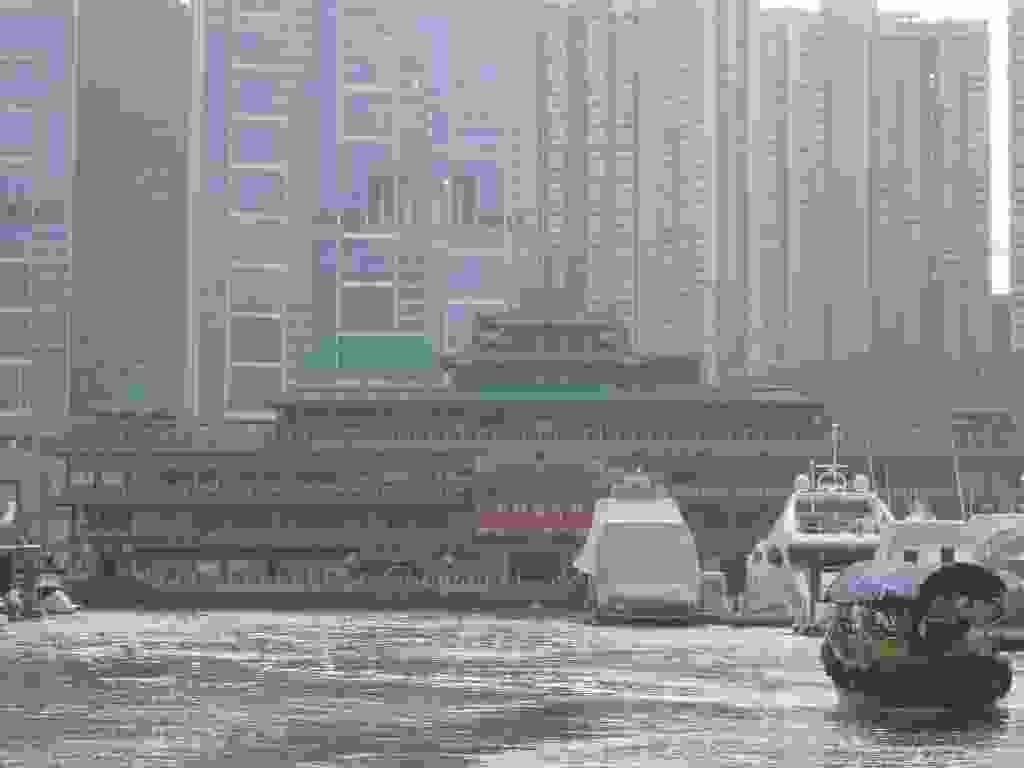
\includegraphics[width=\mywidth]{../wp-content/uploads/2015/10/wpid-oi000106-1024x768.jpg} \end{center}
\vspace{-\topsep}
\pagebreak

  Petit temple, je ne sais pas si c'est bouddhiste ou taoïste. 
\begin{center} 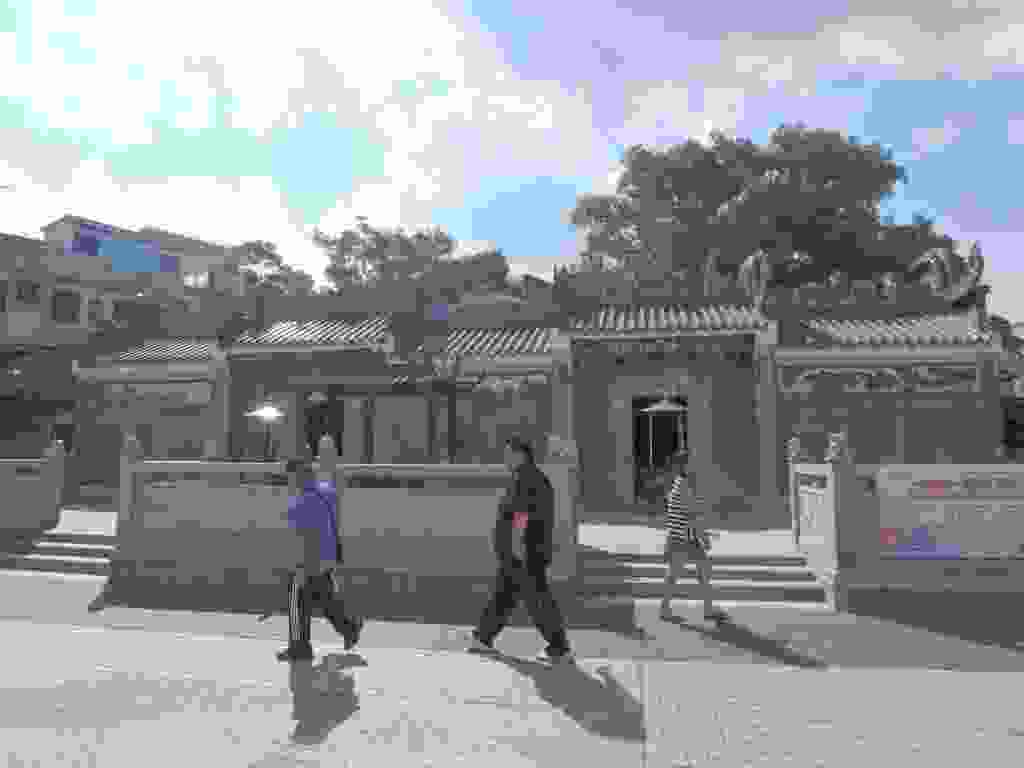
\includegraphics[width=\mywidth]{../wp-content/uploads/2015/10/wpid-oi000066-1024x768.jpg} \end{center}
\begin{center} 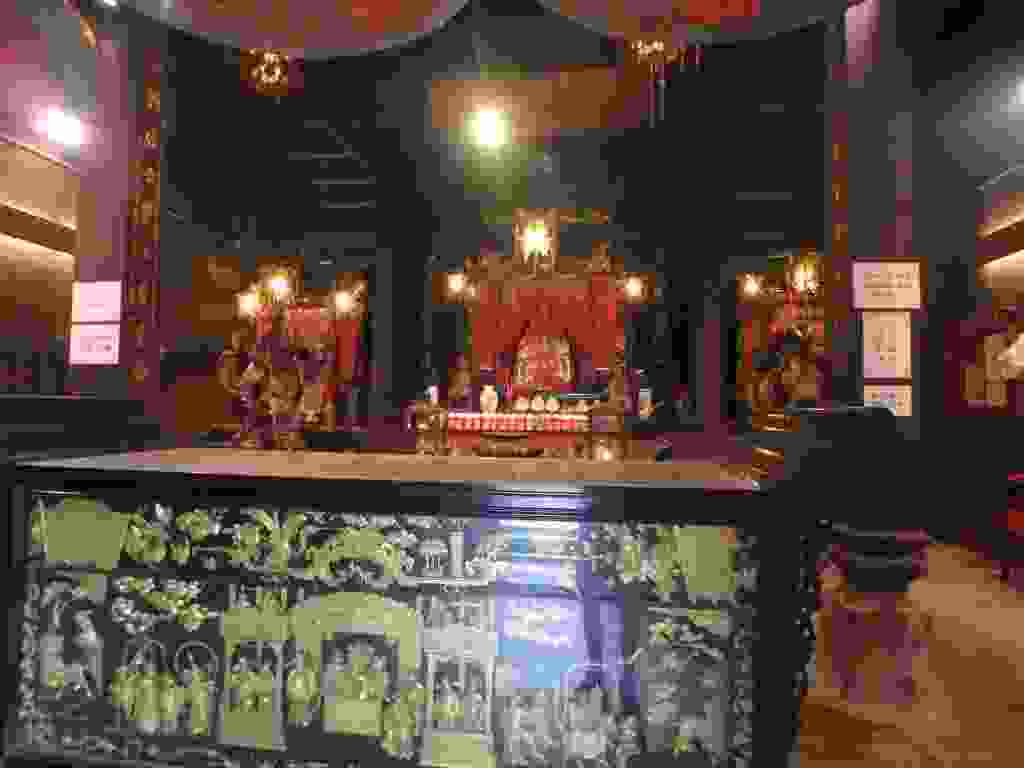
\includegraphics[width=\mywidth]{../wp-content/uploads/2015/10/wpid-oi000092-1024x768.jpg} \end{center}
\vspace{-\topsep}
\vspace{-3.25mm}
\pagebreak
 
 Le long de la rivière entre Hong Kong Island et Kowloon. 
\begin{center} 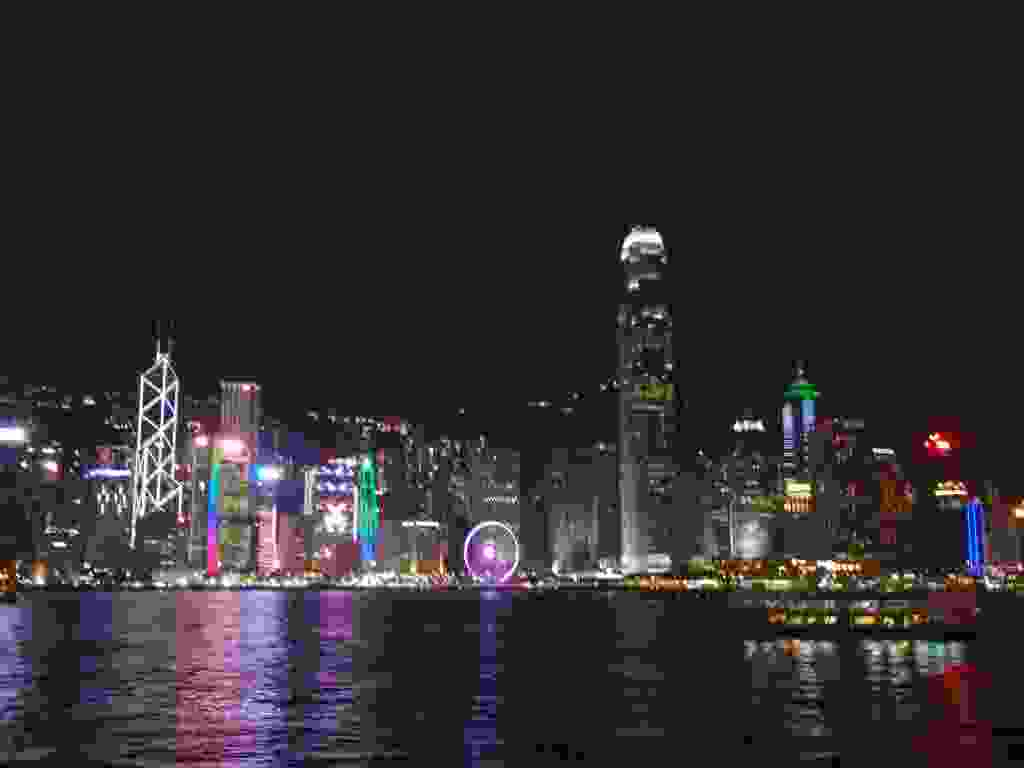
\includegraphics[width=\mywidth]{../wp-content/uploads/2015/10/wpid-oi000072-1024x768.jpg} \end{center}
\begin{center} 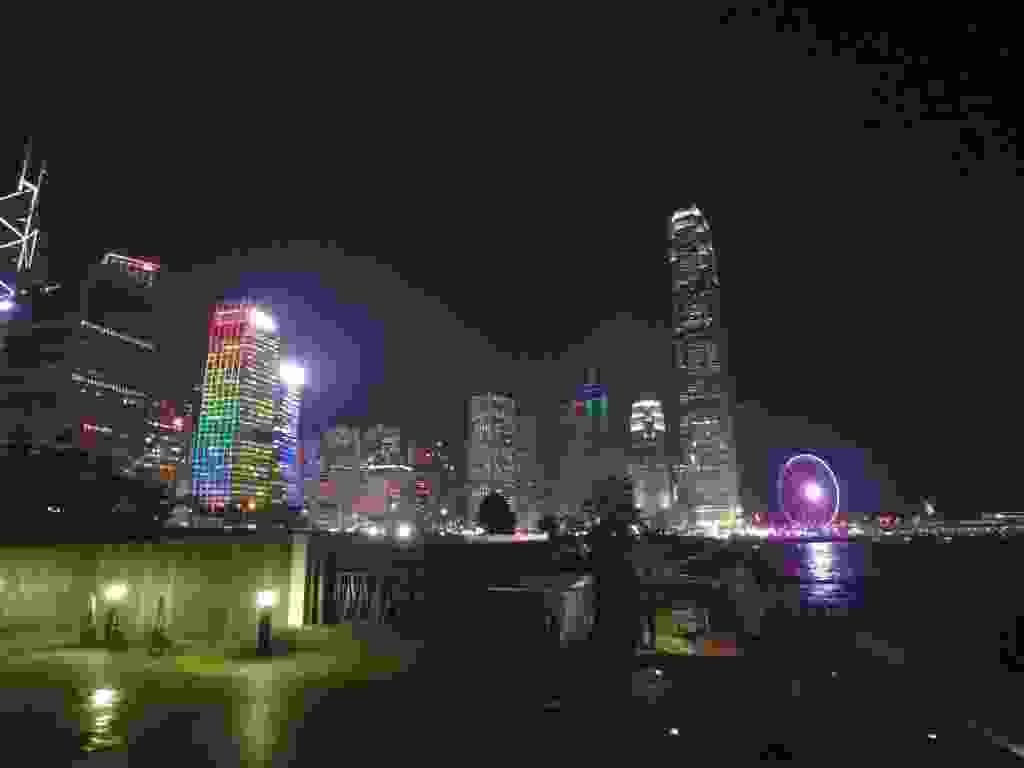
\includegraphics[width=\mywidth]{../wp-content/uploads/2015/10/wpid-oi000113-1024x768.jpg} \end{center}
 \vspace{-\topsep}
 \vspace{-3.25mm}
 \pagebreak
 
 Traversée de Hong Kong Island d'ouest en est en tramway. 
\begin{center} 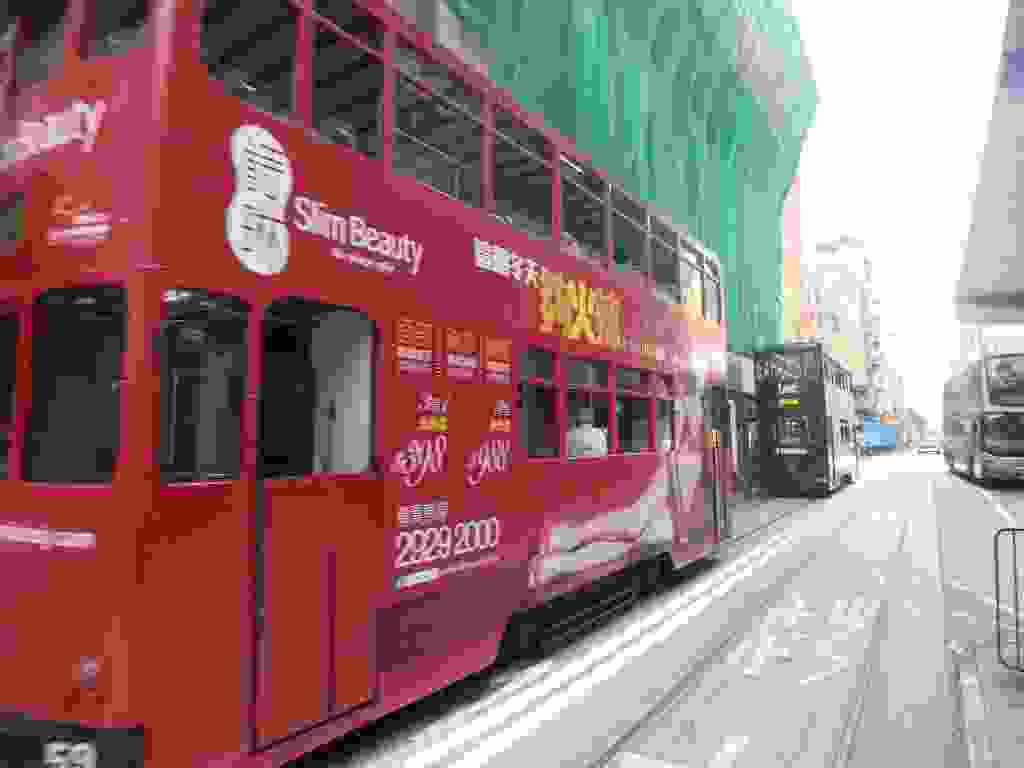
\includegraphics[width=\mywidth]{../wp-content/uploads/2015/10/wpid-oi0000741-1024x768.jpg} \end{center}
\begin{center} 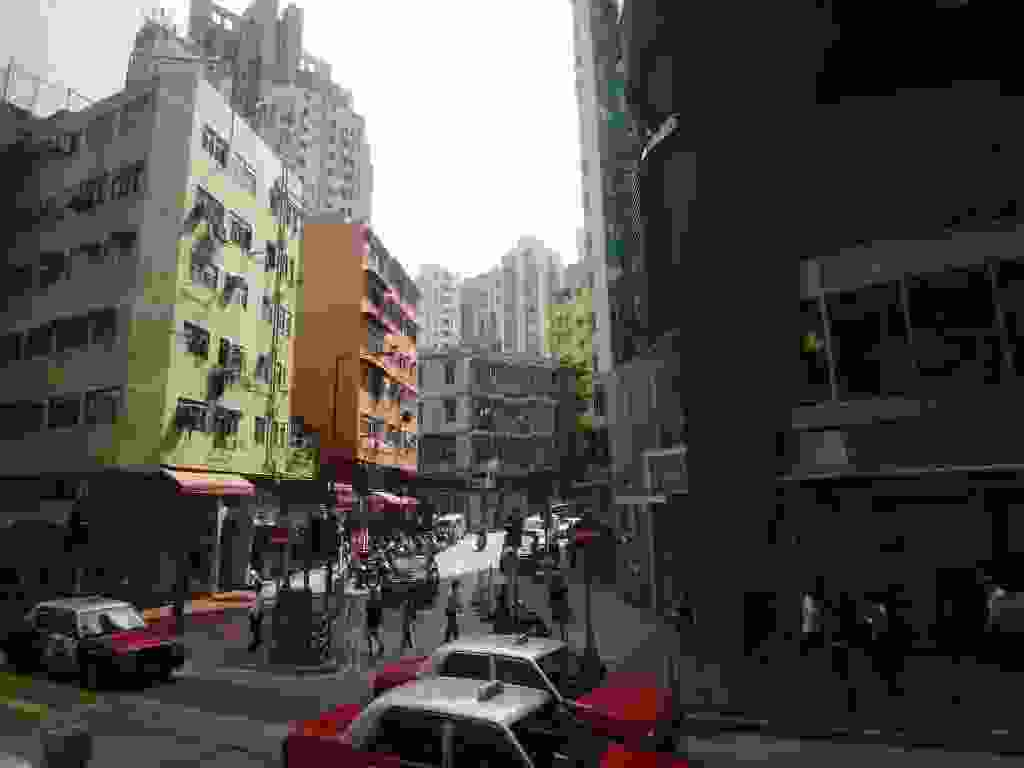
\includegraphics[width=\mywidth]{../wp-content/uploads/2015/10/wpid-oi000087-1024x768.jpg} \end{center}
\begin{center} 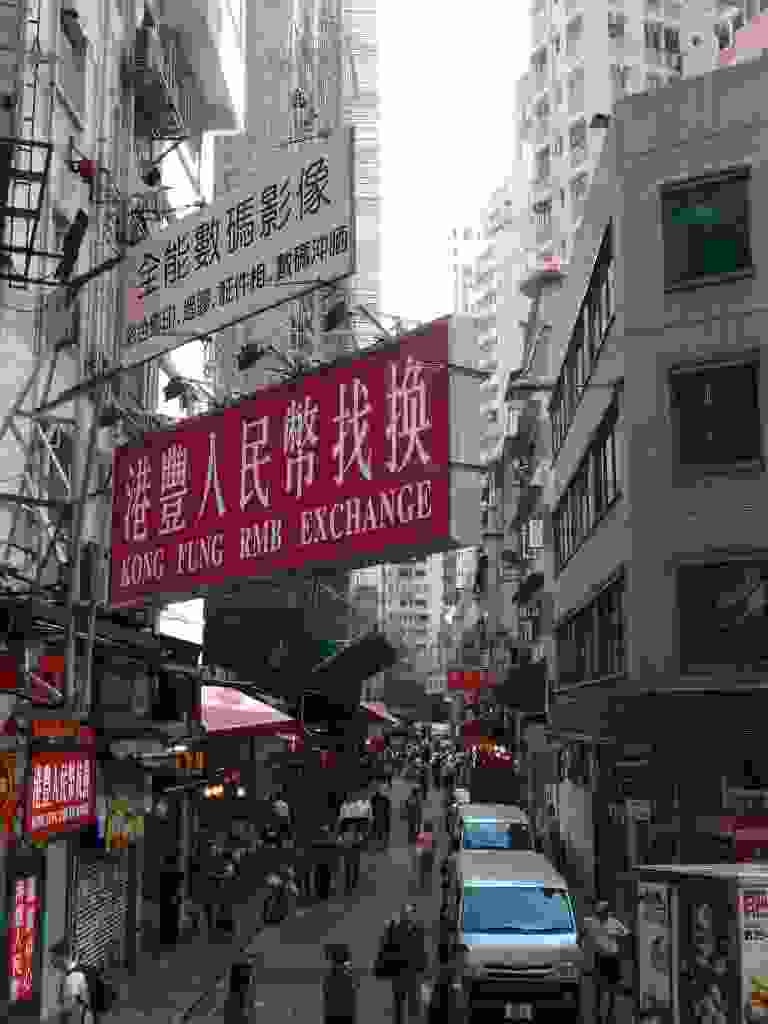
\includegraphics[height=\mywidth]{../wp-content/uploads/2015/10/wpid-oi0000801-e1446026450126-768x1024.jpg} \end{center}

 Dernier jour sur Lantau Island pour voir le grand Buddha en bronze. 
\begin{center} 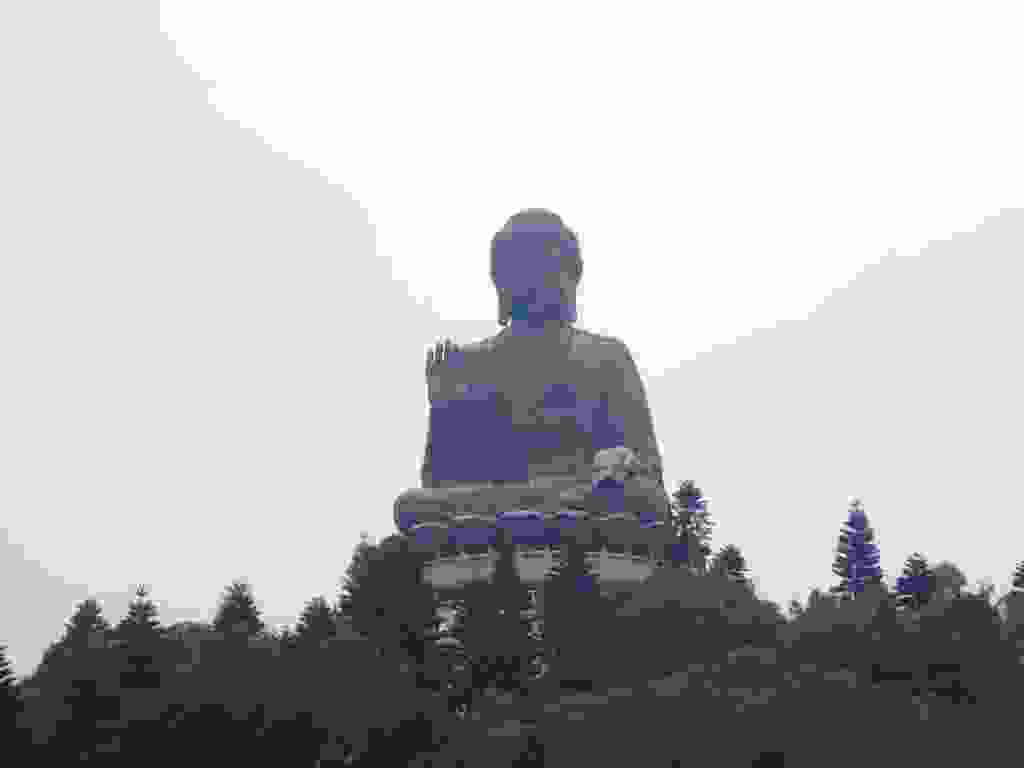
\includegraphics[width=\mywidth]{../wp-content/uploads/2015/10/wpid-oi0001371-1024x768.jpg} \end{center}
\vspace{-\topsep}
\pagebreak

~

\begin{center} 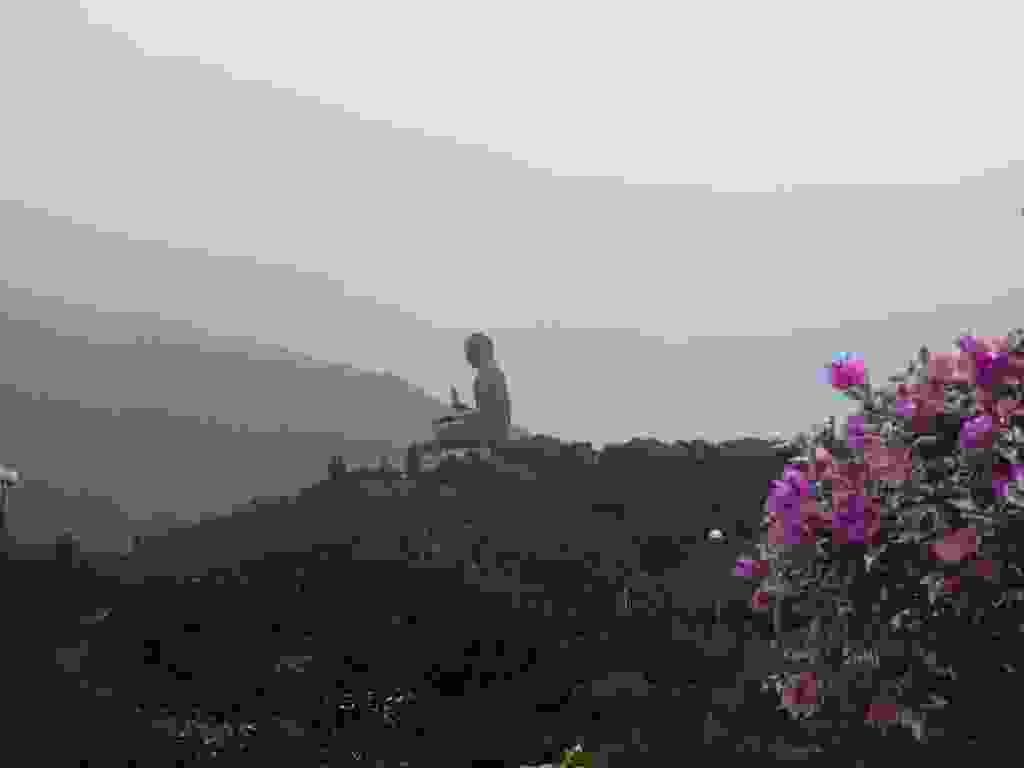
\includegraphics[width=\mywidth]{../wp-content/uploads/2015/10/wpid-oi0001411-1024x768.jpg} \end{center}
\vfill
\begin{center} 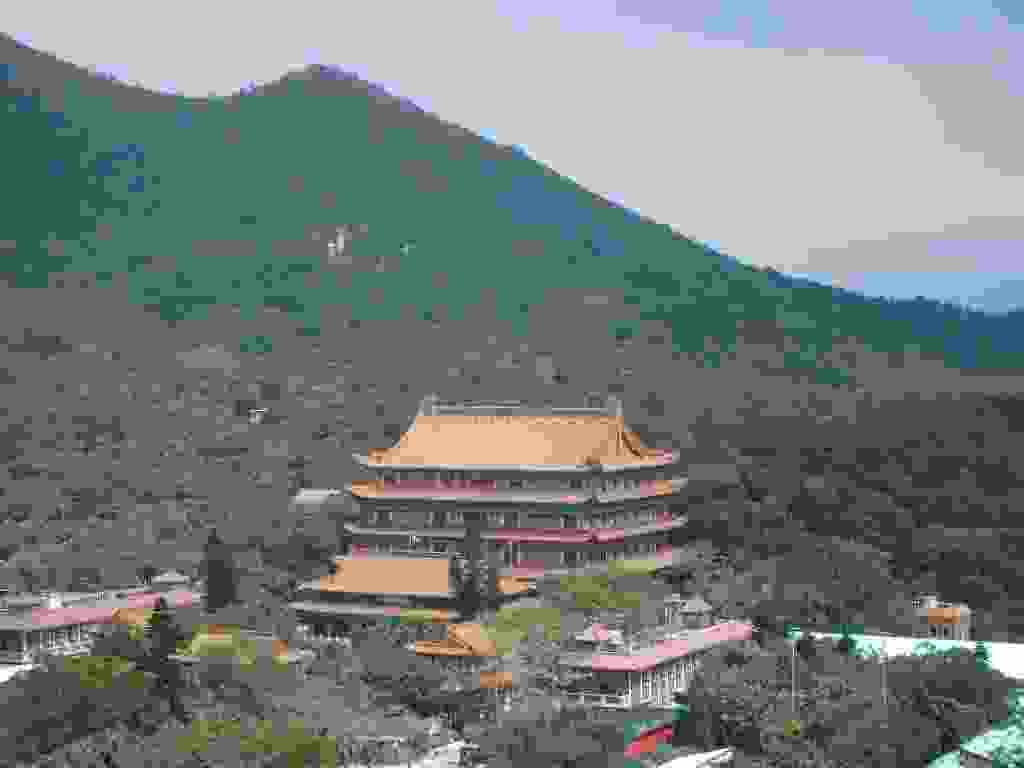
\includegraphics[width=\mywidth]{../wp-content/uploads/2015/10/wpid-oi0001301-1024x768.jpg} \end{center}
\vspace{-\topsep}
\vspace{-0.75mm}
\pagebreak

  Métro pour aller à l'aéroport, destination le sud de l'Inde. 
\begin{center} 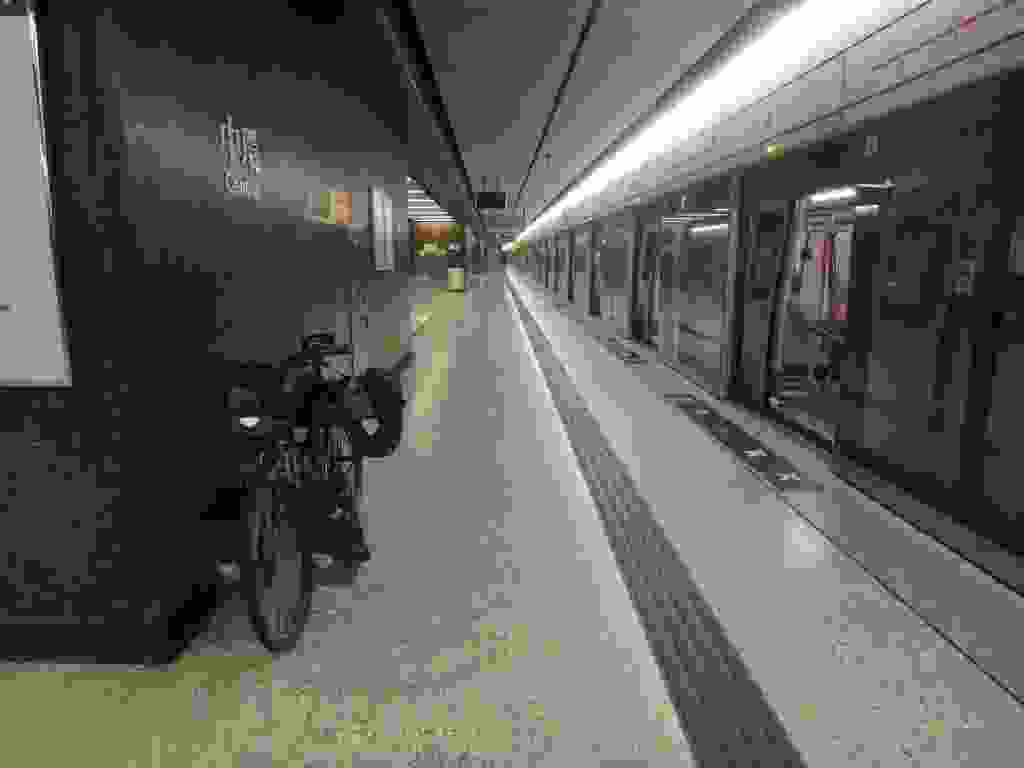
\includegraphics[width=\mywidth]{../wp-content/uploads/2015/10/wpid-oi0001431-1024x768.jpg} \end{center}
